% !TeX root = ../main.tex
% Add the above to each chapter to make compiling the PDF easier in some editors.

\chapter{Experiments}\label{chapter:experiments}

This thesis uses the BERTopic model to apply topic modeling on the \#Secim2023 dataset. 
Before diving into the results and discussion, this chapter explains the dataset, 
how the tweet hydration\footnote{The process of retrieving a tweet's complete information
with only tweet ID.} is performed on the tweets from the dataset, how BERTopic and 
neural topic modeling works generally.

\section{The Dataset}

The dataset published by \textcite{secim2023} consists of tweet IDs collected daily 
between July 2022 and June 2023, a total of around 250 million tweets. 
The frequency of the collected tweets is shown in \autoref{fig:collected_tweets}.

\begin{figure}[htb]
    \centering
    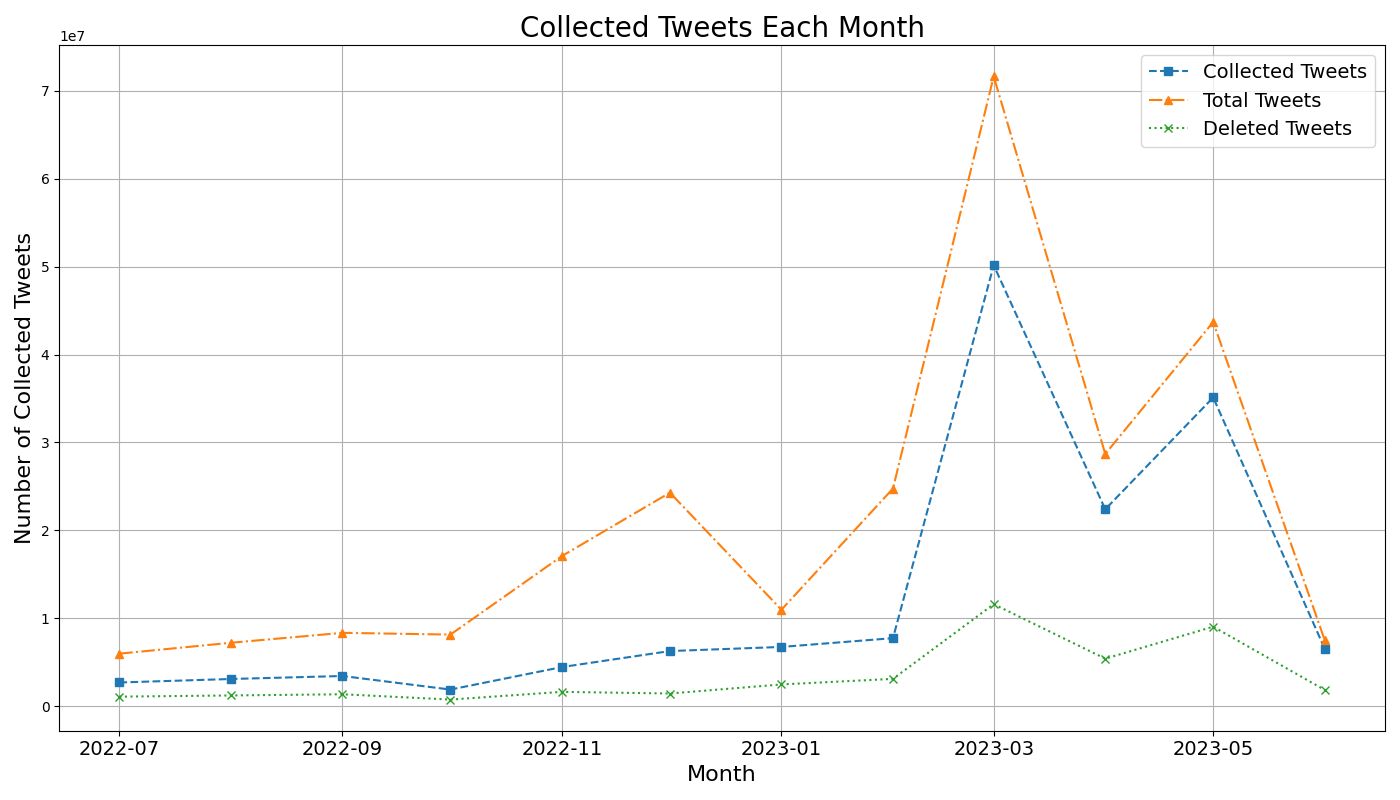
\includegraphics[width=\linewidth]{figures/collected_tweets_2.png}
    \caption[Collected Tweets each month]
    {Number of collected tweets from \#Secim2023 database monthly from July 2022 to June 2023.
    The orange line displays the total number of tweets in the database, 
    the blue line displays the total number of collected tweets from the database and 
    the green line displays the deleted tweets on the month of hydration, around
    December 2023.}\label{fig:collected_tweets}
\end{figure}

Due to Twitter's Developer Agreement and Policy\footnote{https://developer.twitter.com/en/developer-terms/agreement-and-policy}, 
a public dataset can only include (tweet) IDs, which must be hydrated to access the 
tweet information. Typically, a year before, a research group would have had access 
to Twitter Academic API\footnote{https://developer.twitter.com/en/use-cases/do-research/academic-research} 
and used packages like Hydrator\footnote{https://github.com/DocNow/hydrator} to gather 
tweet information. Unfortunately, after Elon Musk bought Twitter, Academic API was 
restricted and then shut down at the end of May 2023, before the start of this 
thesis \parencite{calma_twitter_academicAPI_elon_2023}. Today, there are only paid 
options starting from 100\$ for 10,000 tweets per month, 0.3\% of what was previously 
available for free access in a single day. 

If one has tweet IDs, other methods exist to hydrate the tweets. 
All of the following methods use some embedded retrieval mechanism to gather 
the tweet information. The first method uses Twitter's official page to 
retrieve embedded posts or videos given the tweet ID\: https://publish.twitter.com. 
The second method, which is also used in this thesis, is implemented by React engineers in-house.
% continue from here

\section{The Methodology}

Due to time constraints and the time plan of this thesis, only the BERTopic model 
is used for topic modeling. Since several methods could be used, it is important 
to mention why BERTopic is used and why the others are not.
\textcite{topic_model_comparison_bertopic_2022} found out that for short and 
unstructured texts like Twitter data, BERTopic can extract contextual information, 
and it offers the most potential compared to different embedding-based topic models like Top2Vec.

% compare with Top2Vec
% advantages and disadvantages of BERTopic
% why not others used?
